\begin{exercise}{Teilchen im Kegelmantel}{10}


  \begin{enumerate}
    \item[a)] Überlegen Sie sich die vorhandenen Zwangsbedingungen, wenn sich ein
    Teilchen auf einem Kegelmantel bewegt (Abbildung \ref{fig:TiK}).
    Formulieren Sie die Zwangsbedingung
    so um, dass $\Phi(r,z) = 0$ gilt. Wie viele Freiheitsgrade existieren
    in diesem System anschlie\ss{}end noch?

    \FloatBarrier
    \begin{figure}
      \centering
      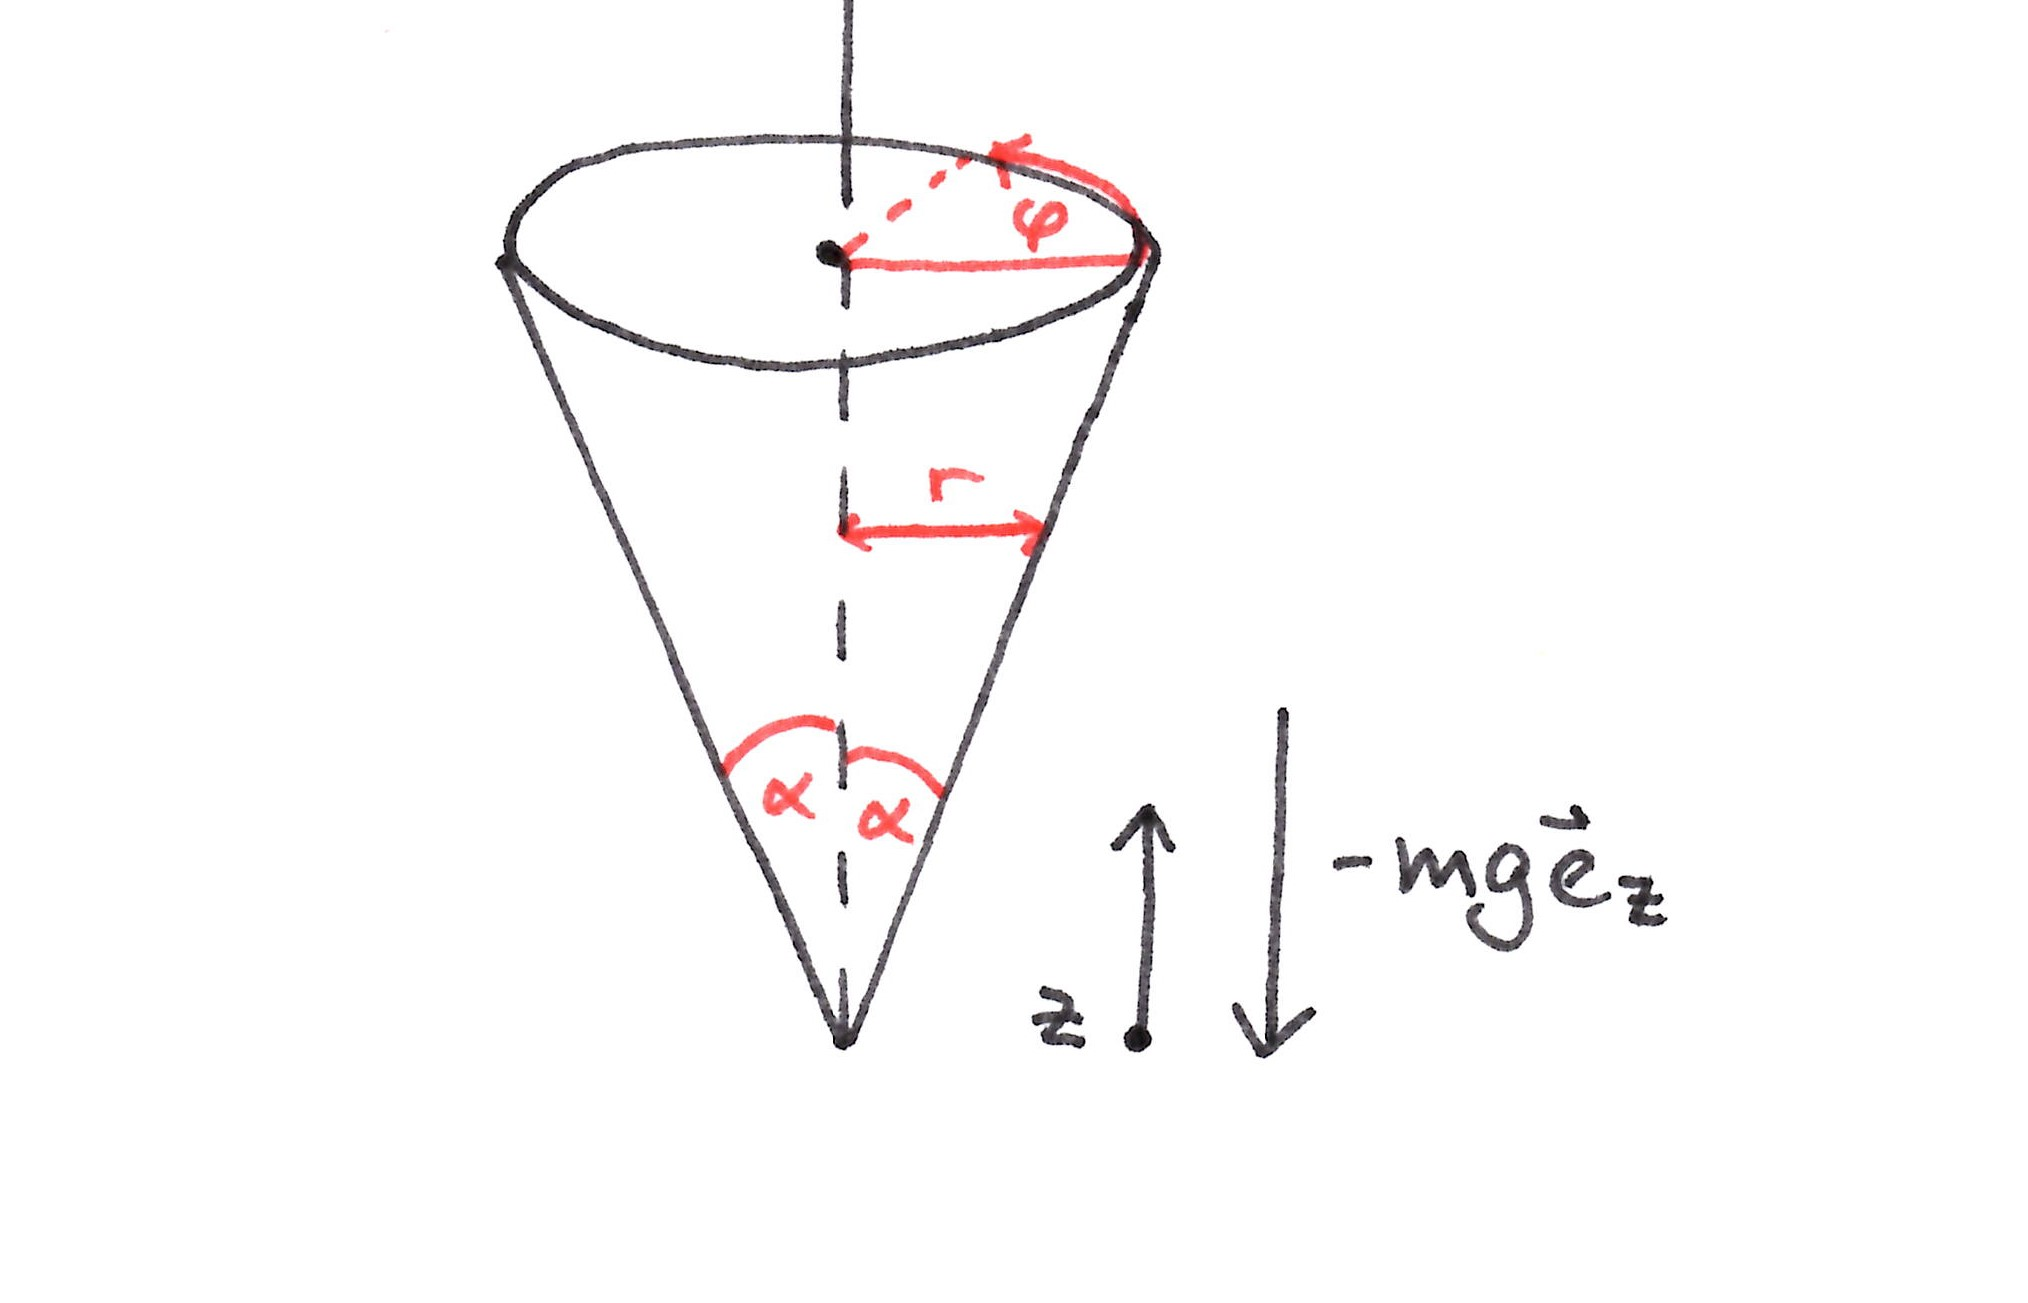
\includegraphics[width = 7 cm]{Kegel.jpg}
      \caption{Teilchen im Kegelmantel.}
      \label{fig:TiK}
    \end{figure}

    \item[\bullet]Durch jede Zwangsbedingung wird die Anzahl der Freiheitsgrade in einem System
    verringert. Um die Richtung der Zwangsbedingungen zu bestimmen, wird dabei
    die Relation $ \vec{\nabla} \Phi \parallel \vec{Z}$ verwendet. Für die
    Zwangskraft wird dann der Betrag $-\lambda$ angenommen, so dass sich

    \begin{equation}
      \vec{Z} = - \lambda \vec{\nabla} \Phi
    \end{equation}

    ergibt. Die Zwangskraft ist die Kraft, die dafür sorgt dass sich das Teilchen
    auf dem Zylindermantel bewegt, steht also senkrecht auf diesen. Wieso ist
    somit auch die Annahme $ \vec{\nabla} \Phi \parallel \vec{Z}$ gerechtfertigt?

    \item[b)] Bestimmen Sie $\vec{Z}$, indem Sie ein geeignetes Koordinatensystem
    verwenden und die oben genannten Relationen verwenden.

    \item[\bullet]In dem am besten geeigneten Koordinatensystem gilt für die Beschleunigung

    \begin{equation}
      \ddot{\vec{r}} = ( \ddot{r}-r\dot{\varphi}^2)\vec{e}_{r} + (r\ddot{\varphi}
      + 2\dot{r}\dot{\varphi})\vec{e}_{\varphi} + \ddot{z}\vec{e}_{z}.
      \label{eqn:Geschw}
    \end{equation}

    Die Newtonsche Bewegungsgleichung lautet für dieses System :

    \begin{equation}
      m \ddot{\vec{r}} = - mg\vec{e}_{z} + \vec{Z}.
      \label{eqn:Newton}
    \end{equation}

    \item[c)] Stellen Sie die Newtonsche Bewegungsgleichung auf, indem Sie
    \eqref{eqn:Geschw} sowie Ihr bestimmtes $\vec{Z}$ in \eqref{eqn:Newton}
    einsetzen. Durch einen Koeffizientenvergleich bezüglich der Terme vor den
    Einheitsvektoren lassen sich 3 Gleichungen formulieren.

    Unter Hinzunahme der
    Zwangsbedingung lassen sich mittels 3 der 4 Gleichungen $\lambda$ und $z$
    eliminieren. Stellen Sie anhand der dann erhaltenden 2 Bewegungsgleichungen
    eine Vermutung auf, welche physikalische Grö\ss{}e in diesem System erhalten ist.
    \\
    \textit{Hinweis: $r\ddot{\varphi} + 2\dot{r}\dot{\varphi} = 0$ wird zum Eliminieren
    von $\lambda$ und $z$ nicht benötigt}

    \item[d)] Betrachten Sie das Problem nun mittels der Euler-Lagrange-Gleichung.
    Überlegen Sie sich, welche zwei generalisierten Koordinaten zu wählen sind
    (siehe vorherige Teilaufgaben) und stellen sie die Lagrange-Funktion auf.

    \item[e)] Ermitteln Sie nun mittels der Euler-Lagrange-Gleichung die Bewegungsgleichungen
    des Systems. Überlegen und Begründen Sie, welche physikalische Grö\ss{}e erhalten
    ist. Wie kann die Erhaltungsgrö\ss{}e auch anhand der Lagrange-Funktion erkannt
    werden? (Begründung anhand der Euler-Lagrange-Gleichung). Welche Auswirkung
    hat die Erhaltungsgrö\ss{}e auf die Bewegung des Teilchens im Kegelmantel?

  \end{enumerate}
\end{exercise}
